% Chapter Template

\chapter{Research Design} % Main chapter title

\label{Chapter3} % Change X to a consecutive number; for referencing this chapter elsewhere, use \ref{ChapterX}

%----------------------------------------------------------------------------------------
%	SECTION 1
%----------------------------------------------------------------------------------------
\section{Research question}
Design projects iterate over designing and investigating and therefore a research question should be formulated. A research question asks for knowledge about the world, without calling for improvement of the world \parencite{Wieringa2014}. By designing a CBM tool for installations at Philips, it has to be investigated what factors play a role. Therefore, answering the following research question will contribute to the knowledge that is necessary to perform this design project:
\begin{center}
\textit{What factors play a role in applying CBM to the Maintenance Decision Making process of RAC RB34?}\\
\end{center}
In Section \ref{Sub-Questions}, sub-questions are formulated that help to answer the research question and achieve the research goal.

\section{Literature review} \label{Literature review}
Currently, maintenance at the RACs is performed after a machine fails or has broken down. This maintenance strategy is called corrective maintenance (CM) and result in costly repairs since the AL have to be shut down abruptly and the production have to be stopped. The maintenance schedule at Philips contains only little information on the average lifetime of equipment. The goal of this project is to design a CBM tool that replaces the CM and improves the maintenance schedule. However, it is possible that in literature other techniques are more applicable to the installations at Philips Drachten. Therefore, other maintenance techniques are discussed in this literature review as well. First, a description of different maintenance activities is given. Thereafter, the two major maintenance techniques widely discussed in literature are described in more detail: time-based maintenance (TBM) and condition-based maintenance.

%\begin{figure}[ht]
%centering
%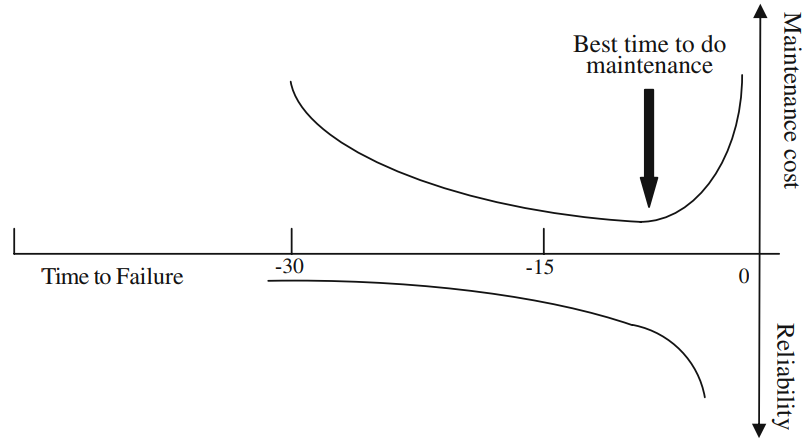
\includegraphics[width=\textwidth, height=7cm]{Figures/bestmaintenance}
%\caption[The relationship between lifetime, reliability, and maintenance cost]{The relationship between lifetime, reliability, and maintenance cost based on \citet{Peng2010}}
%\label{fig:bestmaintenance}
%\end{figure}
\subsection{Introduction to maintenance} \label{Introduction to maintenance}
This introduction to maintenance gives an overview of different possible maintenance activities and is based on lecture nodes for the course Maintenance Planning and Optimization given by Bram de Jonge at the University of Groningen \parencite{DeJonge2017}. 

Organizations are relying more and more on expensive production equipment and therefore the importance of performing maintenance is growing. Buying new machines when old ones are broken down becomes too expensive. Nowadays, organizations realize that efficiency and reliability can be improved if maintenance actions are planned more effectively. As a result, the portion of employees working in maintenance is increasing. From a third of the chemical industry employees to a quarter of the process industry employees deal with maintenance operations \parencite{WAEYENBERGH2002}. Therefore, companies in production industries can significantly increase profits by avoiding unplanned stoppages and bad quality production \parencite{ALSYOUF200}. 

Maintenance can be defined as:
\begin{center}
\textit{'All activities necessary to restore equipment to, or keep it in, a state in which it can perform its designated functions'} \parencite{DeJonge2017}.
\end{center}
From this definition it can be deduced that there are two types of maintenance, that is restore equipment or keep it in state. As mentioned before, maintenance performed after a failure or breakdown is called corrective, reactive, or failure-based maintenance. Maintenance performed before a failure or breakdown when the equipment is still functional is called preventive maintenance and aims to prevent or postpone failures. Preventive maintenance is mostly preferred since it can prevent safety issues, machine damage, quality issues, machine unavailability, long repair times and other unplanned maintenance actions. However, performing maintenance too often result in undesirable cost and therefore a balance between preventive maintenance and risk of failure has to be found. In Figure \ref{fig:Maintenance overview} a schematic overview of maintenance strategies is depicted. Preventive maintenance can be divided into TBM, CBM, and Opportunistic maintenance. 

\begin{figure}[ht]
\centering
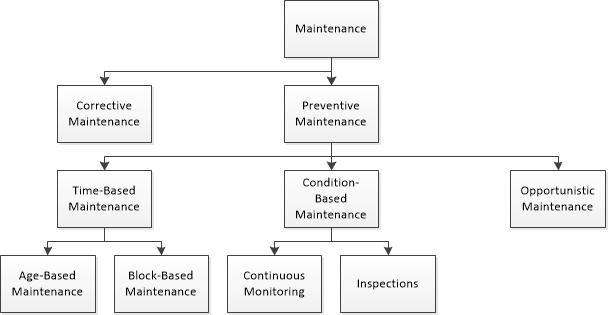
\includegraphics[width=\textwidth]{Figures/Maintenance}
\caption[Schematic overview maintenance strategies]{Schematic overview maintenance strategies based on De Jonge\parencite{DeJonge2017}}
\label{fig:Maintenance overview}
\end{figure}

TBM only depends on the time (age or number of time blocks) that a unit is in service and is therefore relatively easy to implement. However, it is possible that the an item is still in reasonable condition when maintenance is performed or is deteriorating faster than expected and need maintenance earlier. CBM, on the other hand, result in maintenance that is performed just before failure and is generally more effective. However, it can only be applied if condition can be monitored by inspections or continuously and if benefits outweigh the efforts and cost required to apply it. By performing a preventive or corrective maintenance action their might be an opportunity to maintain other units as well. In such cases, the maintenance strategy is called opportunistic. TBM and CBM will be discussed in the next sections, opportunistic maintenance will not be part of this thesis since it can always be combined with another maintenance strategy later. 

\subsection{Time-based maintenance} \label{TBM}
\citet{Yam2001} describe TBM, also known as periodic preventive maintenance, as a traditional maintenance technique. In TBM, maintenance decisions such as preventive repairs are determined based on the estimated expected lifetime of equipment. The expected lifetime is obtained from analyzing the failure behavior of the equipment and, generally, can be displayed as a bathtub curve, Figure \ref{fig:bathtubcurve}. The bathtub curve is divided into three phases: burn-in, useful life, and wear-out. TBM can be introduced to this curve in two steps: The first step is to start with failure data analysis around the left dashed line, the second step is the maintenance decision making at the right dashed line. A complete description of the phases and steps is described by \citet{AHMAD2012}.
\begin{figure}[ht]
\centering
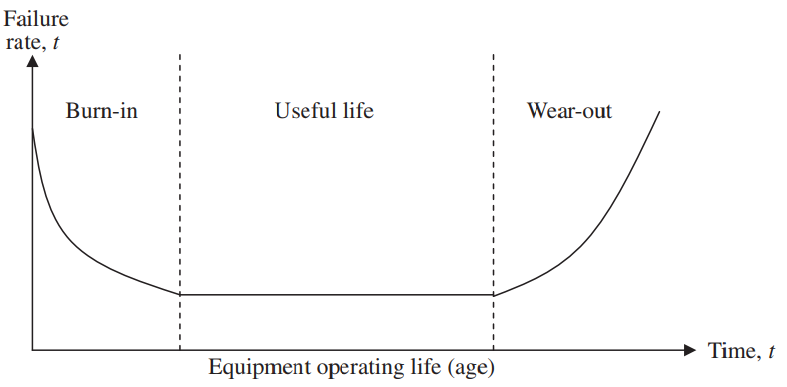
\includegraphics[width=\textwidth]{Figures/bathtubcurve}
\caption[General bathtub curve relation between operating life and failure rate of equipment]{General bathtub curve relation between operating life and failure rate of equipment}
\label{fig:bathtubcurve}
\end{figure}

\citet{GUSTAVSSON2014} consider the scheduling of TBM activities for several components dealing with common set-up costs shared by the components. The gains are combined with the extra costs so that it can be determined if a certain maintenance activity is profitable. TBM contains a number of parameters, such as average lifetime, whose values are optimized numerically or analytically.  However, these parameters are not related to the condition of components but to the estimated lifetime of it. A component far from average can therefore result in performing maintenance too early or too late. A maintenance strategy that is related to the condition of components is discussed below.

\subsection{Condition-based maintenance} \label{CBM}
CBM is thoroughly discussed in literature \parencite{Han2003,AHMAD2012} and is a maintenance program that recommends maintenance decisions based on the condition of equipment and installations. According to \citet{Bloch1983}, 99\% of all machine failures are preceded by certain signs, conditions, or indications that a failure was going to occur. By implementing closed loop maintenance control, sensor feedback information from assembly installations and equipment is utilized in making maintenance-planning decisions. Moreover, continuous collection and interpretation of data regarding the equipment conditions can predict time to failure and an appropriate decision strategy can be applied \parencite{Mann1995}. Firstly, data from various parameters is measured and interpreted continuously, such as vibration, temperature, oil composition, power, and noise levels, which is called the condition monitoring process. This result in maintenance that is performed  just before failure, or just in time (JIT). Secondly, the knowledge of failure causes, effects and deterioration patterns of equipment is increased. Within CBM, diagnostics and prognostics are two important aspects where diagnostics are used for detection, location and identification of faults that occur and prognostics are used to predict the faults before it occurs \parencite{JARDINE2006}. Furthermore, \citet{JARDINE2006} and \citet{Goyal2017} describe that a CBM program consists of three key steps that will be elaborated on briefly: Data acquisition, Data processing, and Maintenance decision making.

\subsubsection{Data acquisition}
Acquiring data is the first step in implementing a CBM program for fault diagnostics and prognostics.  This data can be categorized into event-data and condition monitoring data. Event-data is a description of what happened, for example breakdown, oil pollution or installation and what is done to restore it, for example repair, preventive maintenance or oil replacement. Condition monitoring data are measurements related to the condition health/state of the equipment and installations. As mentioned above there is a wide variety of possible condition monitoring data with as many sensors. The data can be obtained continuously or by inspections. Within seconds, \citet{Golmakani2011} describe an age-based inspection approach where at each step, based on the age of the system, the best time for next inspection is determined. Furthermore, wireless technologies, such as Bluetooth, result in a cost-effective solution to data communication and computerized maintenance management systems (CMMS) are developed for data storage and handling. 

\subsubsection{Data processing}
After the acquisition of data it have to be processed. First, the data is cleaned from any noise preventing it from containing errors, see Section \ref{Data cleaning}. Nevertheless, data cleaning is more applicable to event-data than condition monitoring data since errors can be caused by human factors. However, for condition monitoring data it is possible that sensor faults result in data errors. In general, this can be cleaned by manual examination of data or graphical tools to find and remove data errors. 

After cleaning, the data can be analyzed by using various models, algorithms and tools that are available in literature to understand and interpret the data. The type of data determines the models, algorithms and tools that are useful and can be categorized into three groups \parencite{JARDINE2006}:
\begin{itemize}
\item \textit{Value type}: Data collected at a specific time epoch for a condition monitoring variable are a single value. For example, oil composition, temperature, pressure and humidity are all value type data.
\item \textit{Waveform type}: Data collected at a specific time epoch for a condition monitoring variable are time series, which is often called time waveform. For example, vibration data and acoustic data are waveform type.
\item \textit{Multidimension type}: Data collected at a specific time epoch for a condition monitoring variable are multidimensional. The most common multidimensional data are image data such as infrared thermographs, X-ray images, visual images, etc.
\end{itemize}
The listed types of data are discussed extensively in literature \parencite{WANG1993,Heger2004,ELLWEIN2002}.

\subsubsection{Maintenance decision making}
The last step of a CBM program is maintenance decision-making and is crucial for taking maintenance actions. As mentioned before, techniques for this process are diagnostics and prognostics. Where prognostics is superior to diagnostics since it can save extra unplanned maintenance cost \parencite{JARDINE2006}. Faults and failures that are not predictable have to be detected by diagnostics. Besides, results from diagnostics can be utilized by prognostics to build a better CBM model. 

How much time is left before a failure occurs given the current machine condition is the most widely used type of prognostics. The remaining useful lifetime (RUL) refers to the time left before observing a failure given the current machine age and condition, and the past operation profile \parencite{JARDINE2006}. The RUL of the subsystem can be determined by the operating history up to time. However, it is necessary to embed this into an appropriate decision model which takes accounts of the cost associated with failure and maintenance \parencite{SCARF1997}. Predicting the RUL involves uncertainty and therefore it must be threated as a probabilistic process in which the predicted RUL is represented by a probability density function (PDF) \parencite{Vogl2016}.

\subsection{Comparison of TBM and CBM} \label{Comparison of TBM and CBM}
Previous sections presented an overview of TBM and CBM techniques, in this section a comparison is made between those two. As mentioned previously, CM is a maintenance technique where equipment is repaired once it is broken and will not be discussed thoroughly in this thesis since this technique is already applied to the assembly lines at Philips. In Table \ref{tab:Comparison CBM and TBM}, the advantages of CBM and TBM are listed in comparison with each other.

%------------------------------------------------------
\begin{table}[ht]
\caption{Comparison of CBM and TBM advantages}
\label{tab:Comparison CBM and TBM}
\begin{tabularx}{\linewidth}{>{\parskip1ex}X@{\kern4\tabcolsep}>{\parskip1ex}X}
\hfil\bfseries Condition-Based Maintenance
&
\hfil\bfseries Time-Based Maintenance\\
\cmidrule(r{3\tabcolsep}){1-1}\cmidrule(l{-\tabcolsep}){2-2}
\begin{itemize}
\item No over-maintenance of assets
\item Downtime only before unpredictable failure
\item Increases asset life cycle
\item Minimal risk management
\item No need for failure time data
\end{itemize}
&
\begin{itemize}
\item No need for condition-monitoring equipment
\item No skilled staff necessary to interpret condition-monitoring data required
\item Inventory planning
\item Reduces unplanned downtime
\end{itemize}\\
\end{tabularx}
\end{table}
%------------------------------------------------------------
Most of the advantages that are listed in the table are discussed in Sections \ref{TBM} and \ref{CBM}. Lack of experience might be a problem for companies that are interested in implementing CBM \parencite{ZIO2013} and is therefore an advantage of TBM. However, once CBM is implemented this lack of experience is eliminated. Furthermore, applying CBM to a production process requires a dynamic scheduling of maintenance activities. Companies have to be able to adopt such flexible planning to the already existing planning methods. Within Philips, the maintenance planning is very minimal and therefore adaptability is not considered as a disadvantage. Furthermore, by monitoring the condition of equipment, risks of failure and breakdown occurrence become minimal.

The difference in relations between costs and reliability of every maintenance strategy can be depicted by a graph, Figure \ref{fig:optimummaintenance}. Due to the high maintenance activity level, TBM has relatively low repair cost and high prevention cost. For CM it is the other way around, repair cost are high when breakdowns occur and there are no prevention cost since maintenance takes place only when equipment fails. CBM makes sure that equipment is utilized at maximum and therefore the optimum lays within this sector. Above explanation only holds in theory, if specific equipment failure cannot be monitored the most efficient model can also depend on TBM or a combination of both strategies. 
\begin{figure}[ht]
\centering
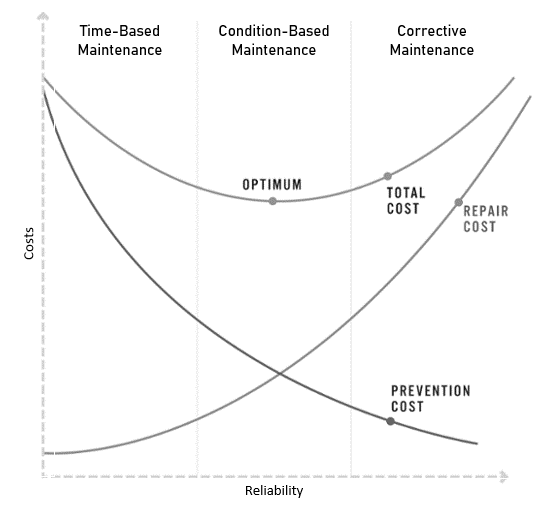
\includegraphics[scale=0.8]{Figures/optimummaintenance}
\caption[Comparison between TBM, CBM and CM]{Comparison between TBM, CBM and CM\footnotemark}
\label{fig:optimummaintenance}
\end{figure}
\footnotetext{https://www.losant.com/blog/using-iot-and-machine-learning-for-industrial-predictive-maintenance}

\subsection{Data cleaning} \label{Data cleaning}
By processing signals from sensors it may occur that a signal suffers unwanted modifications during capture, storage, transmission, or processing, called 'noise'. According to \citet{Ghasemi2010} also errors of measurements and interpretation due to limited accuracy of measurement instruments can cause noise. This noise have to be filtered because it limits the ultimate performances that can be obtained from a given device in terms of signals \parencite{BORDONI1990}. What type of noise occurs depends on the available sensors within a machine but mostly concern temperature, pressure, displacement, weak force, and voltage.

As mentioned before, noise should be eliminated from the equipment condition sensor measurements. In literature, various techniques are described that can separate this noise from actual sensor data. \citet{LESON2016} make use of a Gaussian noise filter, \citet{KALLEN2005} describe a Monte Carlo method and \citet{LU2013} a Quasi Monte Carlo method using the Genz transform to reduce the calculating time and obtain smaller errors. Furthermore, \citet{Bourdin2011} describes a non-local averaging method, that can be used in the frequency domain. Which method is chosen to eliminate the noise depends on the type of sensors that is used with their corresponding signal types.
%Other literature that might be handy to study extensively: 
%\begin{itemize}
%\item Probability distributions - books available at university library
%\item Markov decision processes - books available at university library
%\item Deterioration processes see \parencite{CHEN2015}, \parencite{Do2015}, \parencite{JARDINE2006}, \parencite{Sloan2000}
%\end{itemize}
%Study on these will only be done if the artifact that will be designed is actual dealing with those subjects. For this conceptual version of the project it is not interesting yet. 

\subsection{Implementing CBM} \label{Implementing CBM}
To implement CBM to an existing production process, several steps have to be taken. In Figure \ref{fig:Method CBM}, a method, based on \citet{maxgrip}, is depicted that shows these steps. Sensor data sets regarding robot arm conditions (temperatures, voltages, torques etc.) should be available from the RAC. This data sets will be matched with the event logs, notes from mechanics about for example replacements and observed faults, in order to see what variables in the sensor data correspond with certain event logs. From here, features/patterns should be detected by analyzing the data. \citet{Jaber2017} gives an overview of various techniques regarding vibrations, noise and Motor Current Signature Analysis (MCSA). Furthermore, \citet{Kahane2007} describes that some idea or hypothesis can be verified by gathering and analyzing data by means of regression analysis. One of these techniques should be applied to analyze relationships between variables. When features or patterns are detected by regression analysis or an other technique, a model can be constructed based on the analyzed relationships of variables. Thereafter, a technique that can be used to train a model is necessary. The techniques listed below are not described extensively. A technique will be chosen and described later in Section \ref{SQ2}. Other techniques, such as Artificial Neural Networks, are complex to implement and will not be considered.
\begin{itemize}
\item \textbf{Fuzzy Logic} is a list of if-then statements, called rules, that can be used for computing with words rather than numbers. Although words are inherently less precise than numbers, their use is closer to human intuition \parencite{FuzzyToolbox}.
\item \textbf{Neuro-fuzzy} is a combination of fuzzy logic and neural networks. Fuzzy systems lack the ability to learn or adjust themselves. However, a system based on a neural network provides a promising approach for condition prediction models \parencite{Zhao2009}.
\item \textbf{Markov decision process} is a model for sequential decision making when outcomes are uncertain \parencite{DeJonge2017}.
\item \textbf{Bayes' Theorem} describes the updating process of the probability density function that represents the uncertainty in the parameters based on available data \parencite{canavos1973}.
\end{itemize}
%https://nl.mathworks.com/videos/predictive-maintenance-with-matlab-a-prognostics-case-study-118661.html?elqsid=1518432272733\&potential\_use=Student
%Other models can be found at https://www.autonlab.org/tutorials
\begin{figure}[ht]
\centering
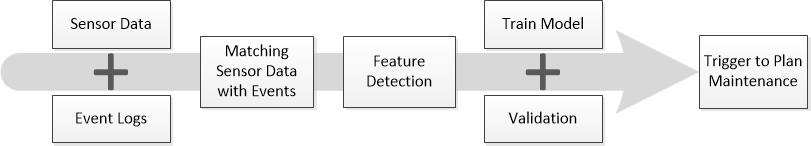
\includegraphics[width=\textwidth]{Figures/CBM_Method2}
\caption[Method of implementing CBM]{Method of implementing CBM}
\label{fig:Method CBM}
\end{figure}

In the ideal situation, CBM is able to detect problems so that equipment can be replaced or repaired before a failure. If the extra CBM related cost are less than or equal to other preventive replacement expenses, no corrective or time-based maintenance is needed \parencite{mckone2002,TAKATA2004}. However, as is described by \citet{ALNAJJAR20003}, CBM may not be 100\% accurate. It is possible that failure occurs before problems are predicted, and on other occasions, conditions will dictate equipment replacement and repair when the equipment could continue to operate for some time. If these prediction mistakes occurs frequently a combination with TBM should be developed where a trade-off between using TBM and CBM is considered.
% zeer handige site http://www-tandfonline-com.proxy-ub.rug.nl/action/doSearch?AllField=A+Failure+Time+Prediction+Method+for+Condition-Based+Maintenance Ook het artikel van Scarf 2007 is erg handig! Verder CTRL+F op scarf in de maintenance library, vrijwel alle artikelen van hem zijn aanraders!

\section{Conceptual Framework} \label{Conceptual Framework}
According to \citet{Wieringa2014}, when the goal is to design an artifact, it have to be ensured that the conceptual framework is understood by the users. The conceptual model for this project consist of three main constructs, Robot Assembly Cell, Maintenance Planning and Users, as is depicted in Figure \ref{fig:conceptual model}. Within every construct elements/functions/activities are defined and the relationships are represented by arrows. The design goal of this project focuses on applying a CBM tool to the Maintenance Decision Making process within the Maintenance Planning. Based on this description of the relations this process has with its environment, sub-questions are formulated in Section \ref{Sub-Questions}. A complete description of the conceptual model is given below:
\begin{figure}[ht]
\centering
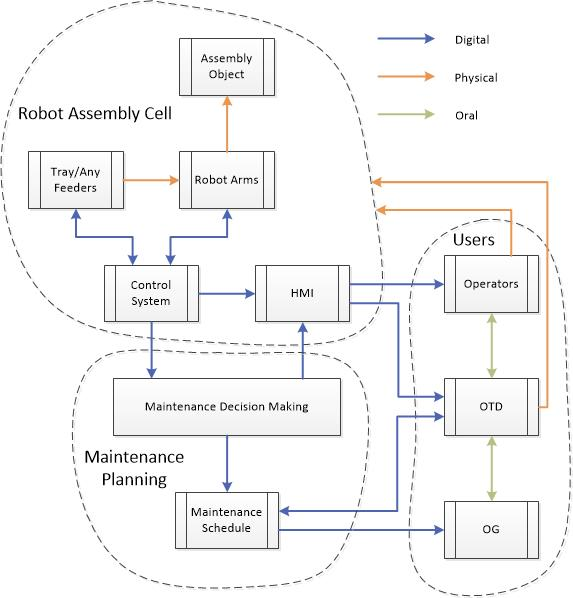
\includegraphics[width=\textwidth]{Figures/Conceptual_Model}
\caption[Conceptual model]{Conceptual model}
\label{fig:conceptual model}
\end{figure}

\begin{itemize}
\item The most important part in the conceptual model are the orange lines within the RAC, those activities determine the throughput of the RAC. Those lines between the \textbf{AnyFeeders}, \textbf{robot arms} and \textbf{assembly object} correspond to the pick and place activities of the RAC, the assembly of holder and springs to the shaver unit. All other activities and streams within the conceptual model are in service of those physical activities. The AnyFeeders ensure product availability for the robot arms so that it can operate continuously. AnyFeeders require less maintenance than the robot arms and therefore only data available from the Robot Arms will be analyzed. 
\item The AnyFeeders and robot arms are controlled by a \textbf{control system}, installed on the RAC computer that assigns tasks. The systems (ACE, V+) that are used to control all RACs at Philips are described in Section \ref{RAC components}. Data from AnyFeeders and robot arms (AC/DC voltages, temperatures, torque, position errors and duty cycles among others) are transmitted to the control system and are displayed by the Human Machine Interface (HMI). Furthermore, the same data is used to decide if maintenance is necessary and is therefore transmitted to the Maintenance Decision Making activity.
\item The \textbf{HMI} provides an interface so that the operators and the OTD can interfere with the control system of the RAC. As mentioned before, data available from AnyFeeders and robot arms can be displayed at the HMI or extracted by connecting an external computer.
\item The \textbf{OTD} and \textbf{operators} consult each other by operating and maintaining the RAC's (green line). The physical repair and maintenance is depicted by the orange lines connecting the OTD and operators with the RAC. The OTD is responsible for maintenance at the RACs and the operators are responsible for operating the entire ALs.
\item Consult takes also place between the OTD and the \textbf{OG}. Employees within those groups determine together if the RAC is working optimal or need maintenance. If maintenance is needed, the OTD provide this maintenance. Members of the OG are described in Section \ref{Stakeholder analysis}
\item This project focuses on designing the \textbf{Maintenance Decision Making} process. This process receives data from the control system and should analyze this data so that it can predict if there is any upcoming maintenance. The output value of this process should than be a \textbf{maintenance schedule} that is constructed automatically for parts where maintenance is predictable. The OTD and OG can take action according to this maintenance schedule. Data analysis should also be displayed on the HMI so that it can be seen what values determined that maintenance should be planned.
\end{itemize} 

\section{Sub-Questions} \label{Sub-Questions}
In order to contribute to the research goal of this project, an artifact have to be designed and sub-research questions can be formulated. In Section \ref{Comparison of TBM and CBM} is concluded that CBM has the highest potential in decreasing maintenance cost. Therefore, sub-questions regarding a CBM tool can be formulated. Furthermore, in Section \ref{Conceptual Framework} it can be seen what elements and relations play a role by improving the maintenance schedule. The sub-questions will be based on the conceptual model regarding these relations. The following questions are formulated with respect to the question constraints described by \citet{Wieringa2014}. \\ \\ 
Sub-question 1:
\begin{center}
\textit{What data types, available from the control system, can predict maintenance activities?}
\end{center}
To design a CBM tool, data that is able to predict upcoming maintenance should be analyzed. Answering this empirical knowledge question will result in a description of the relationship between data and the maintenance it might predict. Literature, expert knowledge and analyzing output data from robot arm can help answering this question. \\ \\
Sub-question 2:
\begin{center}
\textit{How can the output data be interpret in order to predict maintenance?}
\end{center}
From question 1 it is determined what data types are relevant by predicting maintenance. It is necessary to investigate how this data should be interpreted in order to make realistic estimations. In other words, answering question 2 result in a designed artifact that can predict upcoming maintenance. \\ \\
Sub-question 3:
\begin{center}
\textit{On what performance indicators should the artifact be evaluated?}
\end{center}
After an artifact is designed, its performance have to be tested and evaluated in order to validate the design. If the artifact is evaluated successful, it have to supply the maintenance schedule.\\ \\
Sub-question 4:
\begin{center}
\textit{What are requirements for software engineers to integrate the artifact in the control system?}
\end{center}
After designing an artifact, software engineers from Beenen have to integrate it into the HMI of the RACs. During the design phase, requirements for this integration should be considered.


